% !TeX root = main.tex

\hypertarget{related-rates}{%
\section{Related Rates}\label{related-rates}}

In many real-world applications, related variables are changing with
respect to a same variable. For example, the volume \(V\) and height
\(h\) of water in a cylindrical tank change with respect to time \(t\).
Such two rates of change, for example,
\(\dfrac{\mathrm{d}V}{\mathrm{d}t}\) and
\(\dfrac{\mathrm{d}h}{\mathrm{d}t}\) are called \textbf{related rates}.

To solve a related rate problem, the following strategy will be helpful.

\textbf{Problem-Solving Strategy: Solving a Related-Rates Problem}

\begin{enumerate}[sepno]
\item
  Assign symbols to all variables involved in the problem. Draw a figure
  if applicable.
\item
  State, in terms of the variables, the information that is given and
  the rate to be determined.
\item
  Find an equation relating the variables introduced in step 1.
\item
  Using the chain rule, differentiate both sides of the equation found
  in step 3 with respect to the independent variable. This new equation
  will relate the derivatives.
\item
  Substitute all known values into the equation from step 4, then solve
  for the unknown rate of change.
\end{enumerate}

\begin{example}

A \(13\)-ft ladder is leaning against a wall. If the bottom of the
ladder slides away from the wall at a rate \(2\) ft/min, how fast is the
top of the ladder slides down the wall when the bottom of the ladder is
\(12\) ft from the wall.

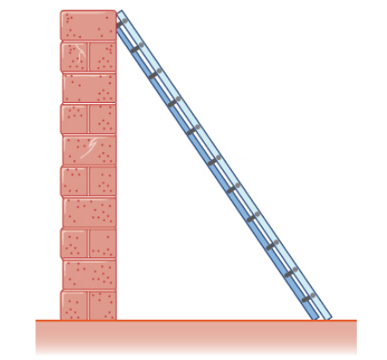
\includegraphics[scale=0.5]{img/image-20201007131231366.png}

\end{example}
\vspace*{6\baselineskip}

\begin{example}

A \(6\)-ft-tall person walks away from a \(10\)-ft lamppost at a
constant rate of \(3\) ft/sec.~What is the rate that the tip of the
shadow moves away from the pole when the person is \(10\) ft away from
the pole?

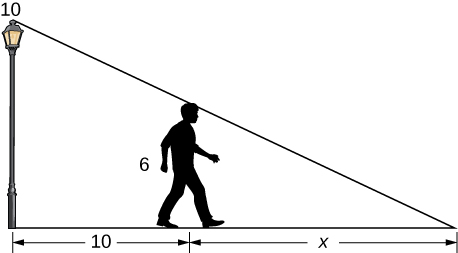
\includegraphics[scale=0.8]{img/CNX_Calc_Figure_04_01_203.jpeg}

\end{example}
\vspace*{6\baselineskip}

\begin{example}

A rocket is launched so that it rises vertically. A camera is positioned
\(5000\) ft from the launch pad. When the rocket is \(1000\) ft above the launch pad, 
its velocity is \(600\) ft/sec. Find the necessary rate of change of the camera's angle 
as a function of time so that it stays focused on the rocket.

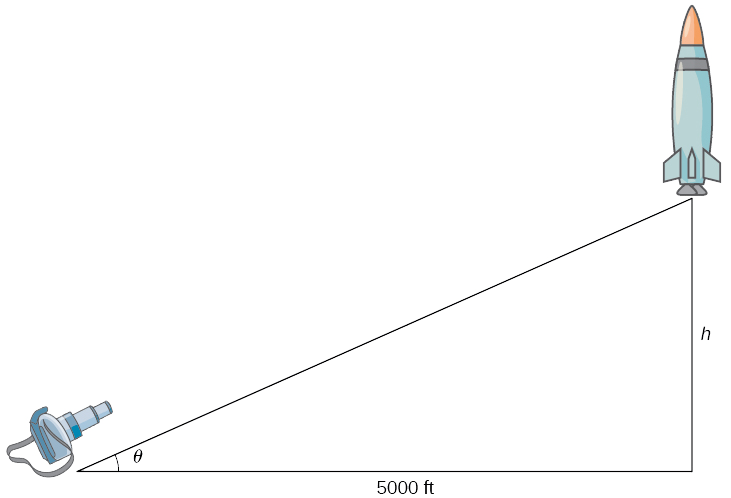
\includegraphics[scale=0.6]{img/4.1.3.png}

\end{example}
\vspace*{6\baselineskip}

\begin{example}

The altitude of a triangle is increasing at a rate of \(1.5\)
centimeters/minute while the area of the triangle is increasing at a
rate of \(5\) square centimeters/minute. At what rate is the base of the
triangle changing when the altitude is \(11\) centimeters and the area
is \(85\) square centimeters?

\end{example}
\vspace*{6\baselineskip}

\begin{example}

A trough has ends shaped like isosceles triangles, with width \(3\) m
and height \(4\) m, and the trough is \(10\) m long. Water is being
pumped into the trough at a rate of \(5\,\text{m}^3\text{/min}\). At
what rate does the height of the water change when the water is \(1\) m
deep?

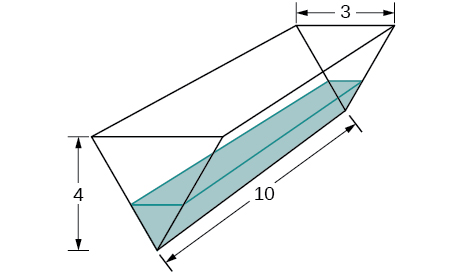
\includegraphics[scale=0.8]{img/CNX_Calc_Figure_04_01_204.jpeg}

\end{example}
\vspace*{6\baselineskip}

\begin{example}

Consider an inverted right cone that is leaking water. (Inverted means the cone's point is facing down, like a funnel.) The dimensions of the conical tank are a height of 16 ft and a radius of 5 ft.

Find the rate at which the surface area of the water changes when the
water is \(10\) ft high if the cone leaks water at a rate of
\(10 \,\text{ft}^3\text{/min}\).

\end{example}
\vspace*{6\baselineskip}

\subsection{Practice}

\begin{exercise}

The volume of a cube decreases at a rate of \(10\) m/sec. Find the rate
at which the side of the cube changes when the side of the cube is \(2\)
m.

\end{exercise}
\vspace*{6\baselineskip}

\begin{exercise}

An airplane is flying overhead at a constant elevation of \(4000\) ft. A
man is viewing the plane from a position \(3000\) ft from the base of a
radio tower. The airplane is flying horizontally away from the man. If
the plane is flying at the rate of \(600\) ft/sec, at what rate is the
distance between the man and the plane increasing when the plane passes
over the radio tower?

\end{exercise}
\vspace*{6\baselineskip}

\begin{exercise}

Two airplanes are flying in the air at the same height: airplane A is
flying east at \(250\) mi/h and airplane B is flying north at \(300\)
mi/h. If they are both heading to the same airport, located \(30\) miles
east of airplane A and \(40\) miles north of airplane B, at what rate is
the distance between the airplanes changing?

\end{exercise}
\vspace*{6\baselineskip}

\begin{exercise}

A circle is inside a square. The radius of the circle is decreasing at a
rate of \(4\) meters per minute and the sides of the square are
increasing at a rate of \(2\) meters per minute. When the radius is
\(4\) meters, and the sides are \(20\) meters, then how fast is the AREA
outside the circle but inside the square changing?

\end{exercise}
\vspace*{6\baselineskip}

\begin{exercise}

A rotating light is located \(14\) feet from a wall. The light completes
one rotation every \(5\) seconds. Find the rate at which the light
projected onto the wall is moving along the wall when the light's angle
is \(15\) degrees from perpendicular to the wall.

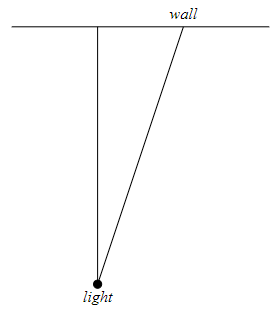
\includegraphics[scale=0.5]{img/image-20201007133107751.png}

\end{exercise}
\vspace*{6\baselineskip}

\begin{exercise}

A cylinder is leaking water but you are unable to determine at what
rate. The cylinder has a height of \(2\) m and a radius of \(2\) m. Find
the rate at which the water is leaking out of the cylinder if the rate
at which the height is decreasing is \(10\) cm/min when the height is
\(1\) m.

\end{exercise}

